\chapter{Analysis Background}
\label{sec:analysis-background}

This chapter provides a comprehensive background on the analysis of language models, tracing the evolution of methods used to understand transformer architectures and their internal representations. We will cover three main areas: historical approaches to analyzing transformers through attention mechanisms, mechanistic interpretability research, and learning dynamics research. This background will set the foundation for the subsequent chapters that explore specific aspects of language model analysis.

\section{Historical Analysis of Transformers through Attention}

The analysis of transformer architectures has historically centered around understanding the attention mechanism, which serves as the primary mechanism for information flow and representation learning in these models. Early work focused on interpreting attention patterns to understand what linguistic phenomena different components of the model were capturing.

\subsection{Multi-Head Attention Analysis}

One of the foundational studies in transformer analysis was conducted by \citet{voita2019analyzing}, who systematically analyzed the role of individual attention heads in transformer models. Their work revealed that attention heads exhibit specialization, with certain heads becoming interpretable for specific linguistic tasks. For instance, they identified heads that specialized in syntactic dependencies, coreference resolution, and discourse relations. This specialization suggested that transformer models develop a form of modular organization where different components handle distinct aspects of language processing.

The findings of \citet{voita2019analyzing} had practical implications for model optimization. They demonstrated that many attention heads could be pruned without significant performance degradation, as only a subset of heads were actively contributing to the model's linguistic capabilities. This insight supported the development of more efficient transformer architectures through selective head pruning.

Building on this work, \citet{michel2019sixteen} conducted an empirical study that further quantified the redundancy among transformer attention heads. Their analysis revealed that while transformer models are typically trained with multiple attention heads, there is significant overlap in the information captured by different heads. This redundancy suggests that the multi-head mechanism, while theoretically capable of capturing diverse attention patterns, often results in redundant representations in practice.

The work of \citet{michel2019sixteen} provided empirical support for the sparsity hypothesis in transformer architectures, suggesting that many attention heads could be removed or simplified without substantial performance loss. This finding has influenced subsequent research on model compression and efficient transformer architectures.

\subsection{Attention Pattern Analysis in BERT}

\citet{clark2019does} pioneered early methods for analyzing attention patterns in BERT, one of the most influential transformer-based language models. Their work investigated what linguistic phenomena different attention heads were attending to, revealing that BERT's attention mechanism captures both syntactic and semantic relationships.

The analysis revealed that certain attention heads in BERT specialized in syntactic phenomena such as subject-verb agreement, while others focused on semantic relationships like coreference resolution. This specialization suggested that BERT's internal representations encode linguistic structure in a distributed manner across different attention heads.

The methods developed by \citet{clark2019does} for visualizing and interpreting attention patterns have become standard tools in the field of transformer analysis. Their work demonstrated that attention weights could serve as a window into the model's internal decision-making processes, providing insights into how transformer models process and represent linguistic information.

\section{Mechanistic Interpretability Research}

While attention analysis provided initial insights into transformer behavior, the field of mechanistic interpretability has developed more sophisticated methods for understanding the internal representations and computations of language models. This research area focuses on identifying specific neurons, circuits, and mechanisms that implement particular linguistic capabilities, with the ultimate goal of achieving full model interpretability.

\subsection{Foundational Concepts in Mechanistic Interpretability}

The theoretical foundation for mechanistic interpretability was established by \citet{olah2014manifolds}, who introduced the concept that neural networks transform data through layers that continuously deform input spaces while preserving their topology. This work supported the manifold hypothesis, which posits that real-world data lies on lower-dimensional manifolds in high-dimensional input space. This framework provides the mathematical basis for understanding how neural networks, including transformers, organize and transform information through their layers.


\begin{figure}[ht!]
    \centering
    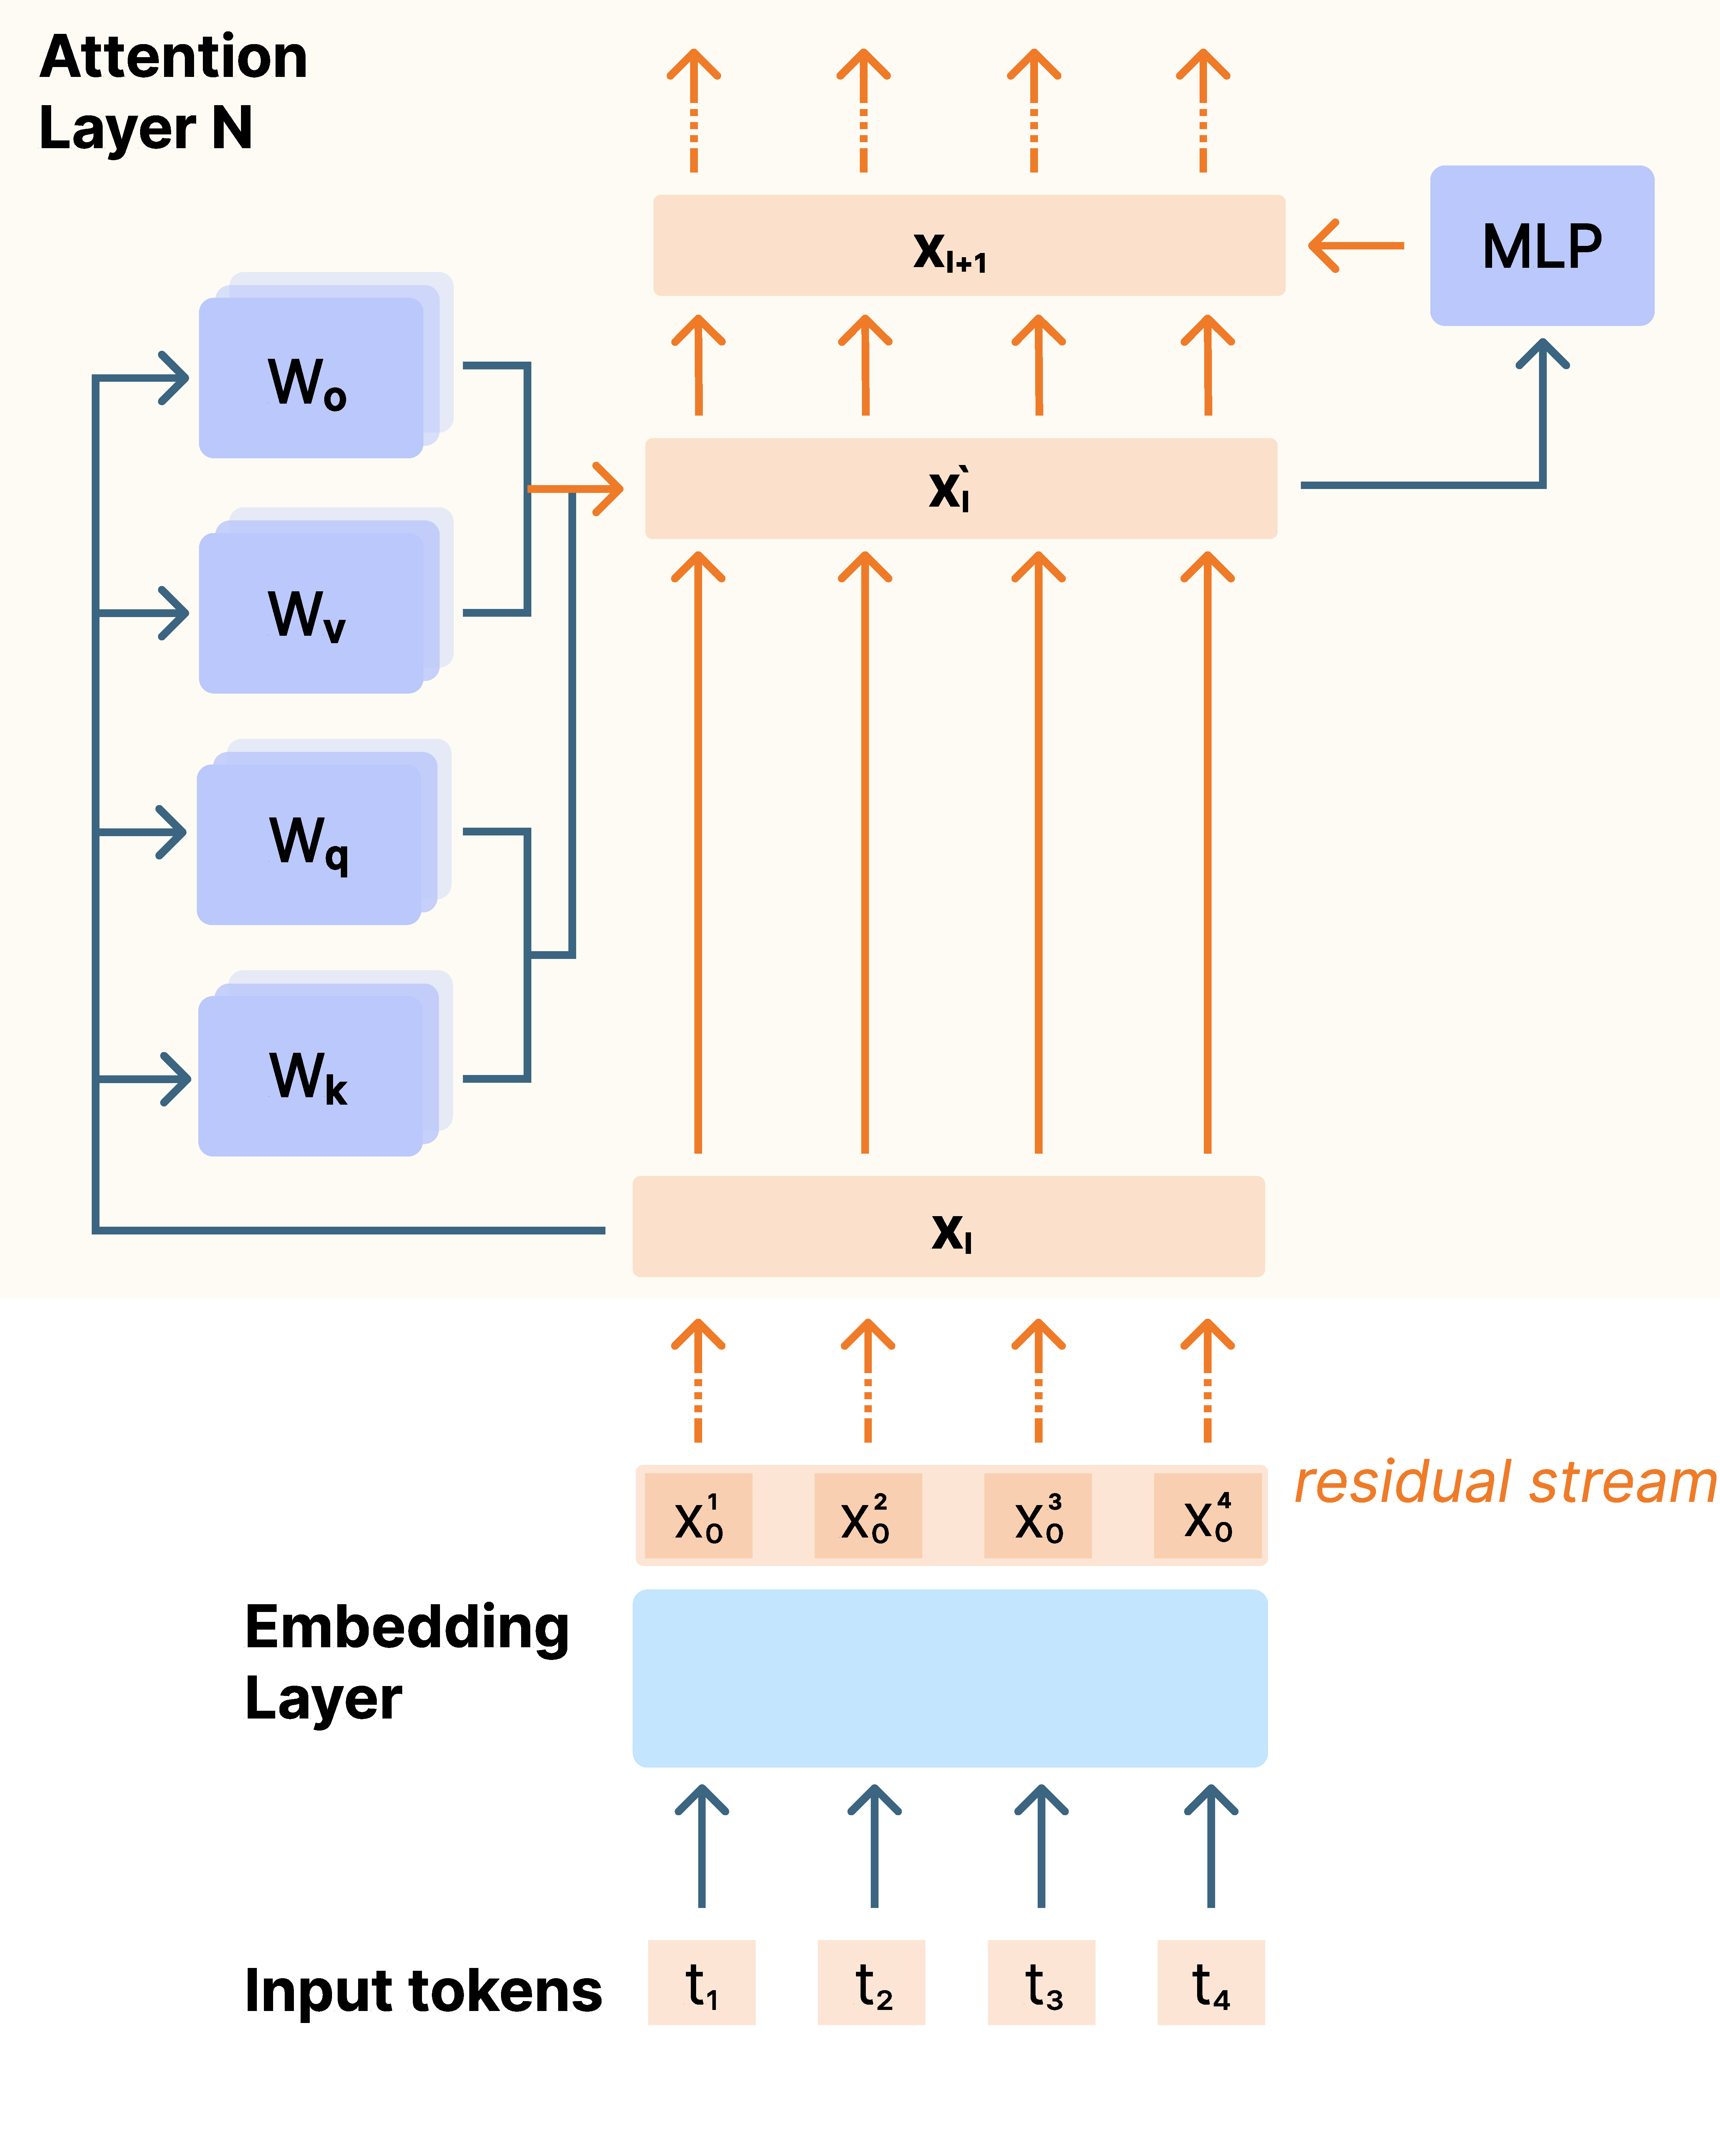
\includegraphics[width=0.6\textwidth]{chapters/analysis_background/figures/residual_stream_visualization.pdf}
    \caption{Visualization of the residual stream in a transformer model, showing how information flows through the network via skip connections and is progressively refined through attention and feed-forward layers.}
    \label{fig:residual-stream}
\end{figure}

\subsection{Circuit-Based Analysis of Transformers}

\citet{elhage2021mathematical} introduced a mathematical framework for understanding transformer architectures through the lens of "circuits" and proposed that transformers can be decomposed into interpretable computational subgraphs. This work developed mathematical tools to analyze attention patterns and their role in computation, showing how attention heads can implement specific algorithms such as copying and induction. The framework introduced the concept of "virtual weights" to explain how attention heads work together, providing a systematic approach to understanding transformer internals.

Building on this circuit-based approach, \citet{olsson2022inductionheads} investigated how transformers perform in-context learning through "induction heads." Their work demonstrated that induction heads are a key mechanism for in-context learning, implementing a specific algorithm for pattern matching. The research provided evidence that induction heads are universal across different transformer architectures and showed how their emergence during training enables various in-context learning behaviors.

\subsection{Superposition and Feature Representation}

\citet{elhage2022toy} introduced a framework for understanding how neural networks represent multiple features in a single neuron through "superposition." This work showed how networks can use superposition to represent more features than dimensions, leading to "interference" between features. The research provided mathematical tools to analyze and understand superposition, demonstrating that it can be both beneficial for efficiency and problematic due to interference. The concept of "sparse coding" was introduced as a way to understand and potentially mitigate superposition effects.

\subsection{Memory Mechanisms in Transformers}

\citet{geva2021memory} proposed that feed-forward layers in transformers act as key-value memory networks. Their work showed that each neuron in the feed-forward layer can be understood as a key-value pair, with these layers storing and retrieving information in a way similar to memory networks. This research provided evidence that feed-forward layers are more important than previously thought and showed how this memory mechanism complements the attention mechanism. The work introduced methods to analyze and interpret the information stored in feed-forward layers.

\subsection{Knowledge Representation and Neurons}

\citet{dai2022knowledge} identified specific neurons in pretrained transformers that encode factual knowledge. Their work showed that these "knowledge neurons" are highly specific to particular facts and that knowledge is distributed across multiple neurons. The research introduced methods to identify and analyze knowledge neurons, demonstrating that they can be used to explain model predictions. The findings provided evidence that knowledge is stored in a way that's both distributed and local, offering insights into how transformers encode factual information.

\subsection{Intermediate Layer Analysis}

\citet{belrose2023eliciting} improved our understanding of how intermediate layers in transformers encode predictive information during generation. Their work generalized the "logit lens" technique by creating a learned diagnostic probe that aligns better with the model's own representations. While the standard logit lens applies the output embedding and softmax to intermediate layer outputs, the tuned lens trains a small set of linear probes to map activations to logits, approximating the final layer's predictions using intermediate activations.

\subsection{Towards Monosemantic Decomposition}

\citet{bircken2023monosemanticity} developed methods for decomposing language models into monosemantic components—neurons or features that correspond to a single, interpretable concept. Their work used dictionary learning (sparse autoencoders) to discover a basis of features from model activations, where each feature corresponds to a sparse, interpretable direction in activation space. The research introduced the concept of monosemanticity, where a component consistently represents one human-understandable feature, and addressed the challenge of superposition where current model activations often mix multiple concepts into a single neuron.

\citet{anthropic2023components} provided a general overview of Anthropic's broader research agenda on mechanistic interpretability, particularly around breaking models into interpretable parts. This work described ongoing efforts toward identifying circuits, features, and neurons that implement human-interpretable behaviors, with the eventual aim of achieving "full model interpretability" where every parameter's role is understood. The research highlighted dictionary learning approaches as promising steps toward faithful model decomposition.

\subsection{Frameworks and Tools for Mechanistic Interpretability}

Several frameworks and tools have been developed to support mechanistic interpretability research. \citet{nanda2022transformerlens} developed TransformerLens, a core library for mechanistic interpretability of transformers that enables detailed inspection of attention heads, MLPs, and circuits. While designed for static model analysis, it provides essential tools for circuit discovery and analysis.

\citet{meng2022locating} introduced ROME, a method for directly editing factual knowledge in transformers. This work built on identifying causal neurons and aligned with post-hoc interpretability approaches, requiring static, trained models for intervention. \citet{conmy2023towards} developed ACDC, which automates the discovery of circuits in transformers using sparse matrix factorization, supporting inference-time interpretability for fixed model weights.

For broader model analysis, \citet{kokhlikyan2020captum} provides a PyTorch library for feature attribution and saliency methods, including Integrated Gradients and DeepLIFT. While less specialized than TransformerLens, it supports a broad class of models and attribution techniques, making it useful for comparative analysis across different architectures.

\subsection{Implications for Language Model Analysis}

The mechanistic interpretability research has profound implications for understanding language models. It reveals that transformers implement sophisticated algorithms through specific circuits and mechanisms, with knowledge distributed across multiple components in ways that balance efficiency with interpretability. The development of tools and frameworks for circuit discovery and analysis has made it possible to systematically investigate the internal workings of these models, moving beyond surface-level attention analysis to deeper understanding of computational mechanisms.

This body of work demonstrates that language models can be decomposed into interpretable components, though the challenge of superposition and the distributed nature of knowledge representation requires sophisticated analysis techniques. The research provides a foundation for developing more interpretable and controllable language models, with applications ranging from model debugging to knowledge editing and safety analysis.

\section{Developmental Interpretability}

While most interpretability research focuses on analyzing fully trained models, developmental interpretability represents an emerging approach that studies models as they train, rather than post-hoc. This paradigm shift enables researchers to understand how linguistic capabilities emerge and develop over the course of training, providing insights into the learning process itself rather than just the final learned representations.

\subsection{Foundational Concepts in Developmental Interpretability}

\citet{hoogland2023towards} proposed studying models as they train, investigating "phase transitions" in learning and representational development. This work introduced the concept of developmental interpretability as a distinct research agenda that focuses on the temporal evolution of model capabilities rather than static analysis of trained models. The approach emphasizes understanding how and when different linguistic phenomena emerge during training, providing insights into the developmental trajectory of language model learning.

A key concept in developmental interpretability is the Local Learning Coefficient, a complexity measure for deep neural networks that quantifies the difficulty of learning specific patterns or representations. This measure provides a theoretical framework for understanding why certain linguistic phenomena emerge at different stages of training and how the learning process progresses through distinct phases.

\subsection{Stagewise Development and Loss Landscape Geometry}

\citet{hoogland2025losslandscape} studied the dynamics of training stages using loss landscape geometry, connecting representational development with degeneracy and flatness in optimization. This work revealed how the geometry of the loss landscape influences the emergence of different linguistic capabilities, providing insights into why learning proceeds through distinct stages rather than continuously.

The research demonstrated that loss landscape degeneracy drives stagewise development in transformers, with different phases of learning characterized by specific geometric properties of the optimization landscape. This finding connects the theoretical framework of developmental interpretability with concrete optimization dynamics, providing a mechanistic understanding of how and why learning progresses through distinct phases.

\subsection{Tools and Frameworks for Developmental Analysis}

\citet{devinterpcode} developed DevInterp, a developmental interpretability toolkit for analyzing model checkpoints throughout training. This library provides tools for checkpoint-based model analysis, enabling researchers to track the evolution of internal representations and capabilities over the course of training. DevInterp complements post-hoc interpretability methods by focusing on the temporal evolution of internal structure rather than static analysis of trained models.

The toolkit emphasizes analysis over intervention during training, providing a framework for understanding how models develop their capabilities without interfering with the learning process. This approach enables researchers to identify critical learning phases, understand when specific linguistic phenomena emerge, and track the development of internal representations throughout training.

\subsection{Implications for Language Model Analysis}

Developmental interpretability provides crucial insights into the learning process itself, complementing other analysis approaches by focusing on the temporal dimension of model development. This approach reveals how linguistic capabilities emerge gradually over the course of training, rather than appearing fully formed in the final model.

The insights from developmental interpretability have important implications for model training and curriculum design. Understanding when specific capabilities emerge can inform decisions about training duration, learning rate schedules, and data presentation order. The identification of critical learning phases can help optimize training efficiency and ensure that models develop the desired capabilities.

Developmental interpretability also provides a bridge between theoretical learning dynamics and practical model development. By connecting loss landscape geometry with representational development, this approach provides mechanistic insights into why certain training strategies are effective and how to design better training protocols.

The combination of developmental interpretability with other analysis approaches provides a comprehensive framework for understanding language models. While mechanistic interpretability focuses on the internal structure of trained models, and learning dynamics research examines various metrics during training, developmental interpretability specifically addresses the temporal emergence of capabilities and the developmental trajectory of learning.

\section{Learning Dynamics Research}

Understanding how language models learn and develop their linguistic capabilities over the course of training has become an important area of research. This work focuses on tracking the emergence of linguistic phenomena during training and understanding the developmental trajectory of language model representations. Learning dynamics research can be broadly categorized into two main approaches: temporal analysis of memorization and influence, and convergence analysis through network similarity measures.

\subsection{Temporal Analysis: Memorization and Influence}

\subsubsection{Influence Functions}

\citet{koh2017understanding} introduced influence functions as a technique from robust statistics to trace model predictions through the learning algorithm and back to training data. This approach identifies training points that are more responsible for a given prediction by perturbing the data input rather than the model itself. The method requires oracle access to gradients and Hessian-vector products, using the result that the influence of upweighting a datapoint on the parameters is given by the inverse Hessian multiplied by the gradient of the empirical risk function with respect to the data point at the current parameters.

Building on this foundation, \citet{grosse2023influence} applied influence functions to large language models to answer counterfactual questions about how model parameters and outputs would change if a given sequence were added to the training set. This work demonstrated the applicability of influence analysis to the scale and complexity of modern language models, providing insights into the relationship between training data and model behavior.

\subsubsection{Forgetting and Memorization Dynamics}

\citet{toneva2019empirical} introduced the concept of forgetting events, tracking when a model flips from correct to incorrect on a given training example during training. This approach provides measures of learning stability and example difficulty, offering insights into the temporal dynamics of learning. While not language-model specific, the methodology has been adapted for NLP applications.

\citet{swayamdipta2020dataset} developed dataset cartography, which measures consistency and variability of model predictions across training epochs. This work applied prediction dynamics to NLP datasets, including BERT fine-tuning, and provided practical applications for understanding dataset characteristics and model learning patterns.

\citet{feldman2020does} explored the memorization-generalization tradeoff using prediction trajectories, discussing example-level dynamics and when memorization is necessary, especially in smaller models. This work provided theoretical insights into the relationship between memorization and generalization in neural networks.

\citet{biderman2023emergent} studied memorization in the Pythia language model family, defining memorization as outputting verbatim training sequences. Their work formulated a forecasting problem: predicting which sequences a large model will memorize using either smaller model runs or early training checkpoints. Key findings included that smaller fully trained models do not reliably predict memorization in larger models, but early checkpoints of the same model do reliably forecast final memorized content, achieving high recall.

\subsection{Convergence Analysis: Network Similarity}

\subsubsection{Canonical Correlation Analysis and Variants}

\citet{raghu2017svcca} introduced Singular Vector Canonical Correlation Analysis (SVCCA), which allows analysis of weight outputs as subspaces without requiring axis alignment. This method enables comparison of representations across different layers and models by analyzing the canonical correlation between their singular vectors.

\citet{morcos2018pwcca} developed PWCCA (Projection-Weighted CCA) to address the noise problem in the original SVCCA approach. They argued that averaging correlations included noise, so instead used a weighted average that rewards signal more heavily when computing the final correlation between singular vectors and original inputs.

\citet{kornblith2019cka} identified limitations of CCA for measuring similarities between representations with higher dimension than the number of data points. They proposed Centered Kernel Alignment (CKA) as an alternative, which learns kernel functions between different inputs to layers of interest and considers how much variance is explained by each input.

\subsubsection{Model Stitching Techniques}

\citet{lenc2015understanding} introduced the concept of stitching layers together in CNNs to reveal structure in the similarity between different layers. This approach provided a new perspective on understanding representation similarity across model architectures.

\citet{bansal2021stitch} formalized model stitching as connecting the bottom layers of one model to the top layers of another with a trainable layer in between. This technique reveals similarity in representations that cannot be captured by CKA and demonstrates that representations trained with more data, larger width, and more training time can improve performance in weaker models.

\subsubsection{Applications to Language Models}

\citet{saphra2019understanding} used SVCCA to show that language model training with ELMo learns similar representations to those of a POS tagger during training, with POS information being learned earlier in the training process.

\citet{nguyen2020wide} used CKA to investigate how neural network representations vary with width and depth. They found that wider and deeper networks develop characteristic block structures in hidden representations, particularly when model capacity is large relative to training set size. These block structures arise when underlying layers preserve and propagate the dominant principal component of their representations.

\citet{singh2019bert} used CCA to demonstrate that multilingual BERT models don't have a universal representation of language. They found that deeper layers diverge in their representations of different languages, with hierarchical clustering revealing tree structures that correspond to phylogenetic relationships.

\citet{phang2021finetuned} used CKA to compare similarity across task-tuned models between layers, finding block structures in the models. They observed that similarity was especially pronounced between later layers, which only marginally contribute to task performance.

\citet{wu2020similarity} analyzed contextual word representation models and found that models in the same family are more similar to one another, while different architectures have similar representations but different individual neurons. This work identified different types of representation similarity across model architectures.

\citet{brown2023understanding} applied metrics like CKA to understand generalization in the Pythia suite, focusing on model comparison post-training rather than training-time convergence. This work emphasized intra-model dynamics during training and provided insights into how different models develop similar or divergent representations.


\subsection{Sparsity and Norms Analysis}

Beyond temporal and convergence analysis, understanding the sparsity of activations and weights, as well as the evolution of various norms during training, provides crucial insights into how language models develop efficient representations and maintain stable training dynamics.

\subsubsection{Sparsity Metrics and Analysis}

\citet{hoyer2004sparsity} introduced Hoyer's sparsity metric, which combines ℓ₁ and ℓ₂ norms to measure sparsity on a continuous scale from 0 (dense) to 1 (maximally sparse). This metric is particularly well-suited for measuring sparsity in activations and feature maps, offering insight into representation compression during training. The metric has been widely adopted in language model analysis to assess when and where sparsity emerges during training.

\citet{hurley2009gini} provided a theoretical framework for evaluating sparsity metrics, proposing six desirable properties that a good sparsity measure should satisfy, including scale invariance, permutation invariance, and continuity. Their analysis showed that the Gini coefficient and Hoyer's sparsity meet all six properties, making them robust and interpretable for analyzing tensor sparsity in neural networks.

\subsubsection{Functional Sparsity in Language Models}

\citet{frankle2019lottery} demonstrated that sparse subnetworks can be trained to full performance, motivating analysis of which parameters remain active during training and which drop out. This work established sparsity as a proxy for overcapacity versus signal alignment, which is particularly relevant for understanding the differences between small and large language models.

Building on this foundation, \citet{michel2019sixteen} showed that many attention heads in transformer models are redundant. Their work demonstrated that language models can tolerate significant sparsity through head pruning during training, providing an interpretability-aligned justification for sparsity metrics in transformer architectures.

\citet{evci2020rigging} examined the training dynamics of sparsified networks, highlighting the instability of sparse networks during early training phases. This work revealed important insights into how sparsity affects the learning process and when it becomes beneficial for model performance.

\citet{voita2019analyzing} introduced head importance scoring and showed that sparsity naturally emerges in attention heads during training. This work provided an excellent case study of functional sparsity in language models, demonstrating how certain attention heads become specialized while others become less important.

\citet{jiang2023pruning} measured activation sparsity and proposed sparsity-aware pruning methods for pretrained transformers. Their work is particularly useful for understanding which neurons become saturated, unused, or dead during training, providing insights into the internal organization of language model representations.

\subsubsection{Norm Evolution and Training Stability}

\citet{mishkin2016goodinit} studied how weight and activation norms evolve during training, with particular focus on layer normalization and gradient scaling in transformers. This work revealed important patterns in how different types of norms change throughout the training process and their relationship to model performance.

\citet{liu2020understanding} investigated activation and gradient norm explosion and vanishing in transformers, highlighting early instability in small models. This research is particularly relevant for understanding convergence challenges in transformer training and identifying when models become unstable during the learning process.

\citet{arora2018theoretical} connected parameter norm growth to generalization bounds, providing theoretical motivation for tracking norm-based proxies during training. While primarily theoretical, this work established important connections between the magnitude of model parameters and their generalization properties.

\citet{zhang2021calibration} investigated the link between logit norms, confidence, and miscalibration in modern neural networks. This work motivates looking at output norm dynamics as a proxy for confidence evolution, providing insights into how language models develop calibrated predictions over the course of training.

\subsubsection{Implications for Language Model Analysis}

The analysis of sparsity and norms provides crucial insights into the internal dynamics of language model training. Sparsity analysis reveals how models develop efficient representations by focusing on the most important components, while norm analysis helps understand training stability and the evolution of model confidence. Together, these approaches complement temporal and convergence analysis by providing fine-grained insights into the internal organization and dynamics of language model representations.

These methods enable researchers to identify when and where sparsity emerges during training, understand the relationship between parameter magnitudes and generalization, and track the evolution of model confidence and stability. The combination of sparsity and norm analysis with other learning dynamics approaches provides a comprehensive framework for understanding how language models develop their capabilities and maintain stable training dynamics.

\subsection{Rank and Geometry Analysis}

The analysis of rank and geometry provides crucial insights into how language models develop their representational capacity and learning dynamics. This approach focuses on understanding the effective dimensionality of model representations and how they evolve during training, revealing important patterns in learning progression and capacity utilization.

\subsubsection{Effective Rank and Learning Progression}

\citet{boix-adsera2023rank} established that during transformer training, the difference between current weights and initialization increases in rank gradually. Their work proved that under small weight initialization, training proceeds in discrete stages, each adding at most one to rank—mirroring incremental learning phases. The empirical evidence showed this effect persists in real transformers, linking rank growth to meaningful learning dynamics. This work established effective rank as a meaningful indicator of learning progress and phase boundaries.

\citet{godey2024small} showed that small language models hit a representational bottleneck due to the softmax layer's rank limits. As training progresses, output capacity saturates even though loss continues to drop, limiting expressivity. This work suggested that small models underperform not due to optimization issues, but due to structural constraints on expressiveness, highlighting output-layer saturation as a measurable failure mode in small models.

\citet{belrose2024neural} demonstrated that networks learn progressively more complex statistical patterns, from unigram statistics to grammar. Training proceeds in stages, with clear shifts in what the model encodes and where (layers, steps). This work provided experimental support for layered learning dynamics and curriculum-like behavior, justifying the use of tools like effective rank or CKA to detect training phase transitions.

\subsubsection{Staircase Phenomena and Phase Transitions}

\citet{yang2024rankstaircase} introduced effective rank to characterize how many principal directions a network uses in its last hidden layer. Their work discovered a staircase pattern where effective rank rises in discrete jumps, closely tracking drops in the loss—indicating phase transitions in learning. This finding provided important insights into how learning progresses through distinct phases rather than continuously.

\citet{garg2025utilizedrank} introduced utilized rank as the number of dimensions in a layer's weight matrix that actually contribute to processing real data. This approach moved beyond full parameter count to measure data-dependent functional capacity. The work identified input/output subspaces via SVD on data passed through the layer and projected weights onto these subspaces. The findings showed that utilized rank is much lower than full rank, with ViT-B/16 using only ~35% of full capacity and ViT-L/16 using only ~20%. Self-supervised pretraining increased utilization, and low-rank approximations preserved accuracy while reducing computational requirements.

\subsubsection{Low-Rank Learning Dynamics}

\citet{pellegrino2023lowrank} showed in recurrent networks that weight matrices evolve along low-rank subspaces throughout training. Both biological and artificial networks displayed low-dimensional connectivity changes during learning, highlighting that rank constraints are a general feature of learning trajectories across architectures.

\citet{feng2022rank} proved that deep neural networks tend toward rank deficiency in hidden representations across layers during training. This work established that the tendency toward low-rank representations is a fundamental property of deep learning systems.

\citet{minyoung2022lowrank} showed that neural networks are biased toward low effective-rank Gram matrices, a signature of structural simplicity in learned representations. This work provided theoretical insights into why neural networks naturally develop low-rank representations during training.

\subsubsection{Implications for Language Model Analysis}

The rank and geometry analysis provides crucial insights into the fundamental learning dynamics of language models. The discovery of staircase phenomena and phase transitions reveals that learning proceeds through distinct stages rather than continuously, with each stage characterized by specific rank increases and loss reductions. The finding that models utilize only a fraction of their theoretical capacity suggests that much of the parameter space in large models may be redundant or unused.

These insights have important implications for model design and training. Understanding rank evolution can help identify when models reach capacity limits and when additional training may not be beneficial. The discovery of low-rank learning dynamics suggests that models naturally develop efficient, compressed representations, which could inform approaches to model compression and efficiency optimization.

The combination of rank analysis with other learning dynamics approaches provides a comprehensive framework for understanding how language models develop their capabilities. Rank analysis complements temporal, convergence, sparsity, and norm analysis by focusing on the fundamental dimensionality and geometry of learned representations, revealing the underlying structure of how language models organize and utilize their representational capacity.

\section{Frameworks and Tools for Learning Dynamics Research}

The study of learning dynamics across different model scales has become increasingly important as researchers seek to understand how scaling affects the emergence and development of linguistic capabilities. Several frameworks and model suites have been developed to support this research, providing standardized datasets, checkpoints, and evaluation tools for studying learning dynamics across scales.

\subsection{Size Comparison and Scaling Studies}

\citet{bansal2021scaling} tracked how model size affects training dynamics, providing crucial insights into how scaling influences learning behavior. This work was particularly helpful for motivating convergence breakdown in small language models and understanding the relationship between model capacity and learning dynamics.

\citet{xia2023training_trajectories} conducted a rare study of full training trajectories using probes and dynamics-focused tools across different model scales. This work provided important baselines for both prediction error reduction (PER) and activation norm analysis, demonstrating how learning dynamics vary systematically with model size.

\subsection{Comprehensive Model Suites}

\citet{biderman2023pythia} developed Pythia, a comprehensive suite for analyzing large language models across training and scale. The suite includes models ranging from 70M to 12B parameters, with 154 checkpoints for each of the 16 models. This extensive dataset enables researchers to study learning dynamics across a wide range of model sizes and training stages, providing standardized benchmarks for comparing different analysis approaches.

\citet{groeneveld2024olmo} introduced OLMo, designed to accelerate the science of language models through comprehensive transparency. The framework releases training checkpoints across multiple hardware types, logs, and datasets, with all model variants trained on at least 2T tokens. OLMo includes 4 variants at 7B scale and 1 variant at 1B scale, along with Catwalk and Paloma for evaluation. The training setup uses ZeRO optimizer strategy with FSDP framework, global batch size of 2048, and sequence length of 2048 with mixed-precision training.

\subsection{Multilingual and Open-Source Frameworks}

The BLOOM (BigScience Large Open-science Open-access Multilingual Language Model) project represents one of the few multilingual models where intermediate checkpoints are available and the training process was fully documented. Models are available from 560M to 176B parameters, with public slices of checkpoints at stages like 0B → 100B → 300B → 500B → 700B → full 1.5T tokens. BLOOM focuses on global participation, multilinguality, and open research scaffolding, making it particularly valuable for studying learning dynamics in multilingual contexts.

\citet{liu2023llm360} developed LLM360, emphasizing radical transparency in open-source language models. The framework includes models at 7B scale with variants like Amber and CrystalCoder. Amber provides 360 checkpoints released approximately every 1B tokens, while CrystalCoder includes 143 checkpoints. The framework includes training logs, loss curves, optimizer states, and model weights, supporting open-source benchmarking, robustness analysis, and interpretability research.

\subsection{Specialized Frameworks for Interpretability}

\citet{thawakar2024mobillama} developed MobiLlama, a lightweight and efficient GPT-style model trained with full transparency. The framework emphasizes training reproducibility and interpretability, with checkpoints and logs released throughout training. This approach supports research on low-resource learning dynamics and mobile deployment tradeoffs, including accuracy vs. sparsity vs. latency considerations.

TinyLlama represents an open-source small language model with 1.1B parameters trained on 3T tokens with full Hugging Face integration. The project publicly releases intermediate checkpoints at 105B, 503B, 1T, 1.5T, 2T, 2.5T, and 3T tokens, providing a standardized dataset for studying learning dynamics in small-scale models.

SmolLM2 provides a suite of small models that outperform other recent small language models, with a 1.7B-parameter LLaMA-style model trained with checkpoints saved every 125K steps. The framework was released specifically for mechanistic interpretability research, providing detailed training trajectories for studying the emergence of linguistic capabilities in smaller models.

\subsection{Implications for Learning Dynamics Research}

These frameworks provide crucial infrastructure for studying learning dynamics across scales, enabling researchers to compare how different model sizes affect the emergence and development of linguistic capabilities. The availability of standardized checkpoints, training logs, and evaluation tools facilitates reproducible research and systematic comparison of different analysis approaches.

The frameworks also support research on scaling laws and the relationship between model capacity and learning dynamics. By providing models across a wide range of scales, from small models optimized for interpretability to large models designed for performance, these frameworks enable researchers to understand how scaling affects the fundamental learning processes in language models.

The combination of these frameworks with the analytical approaches discussed throughout this chapter provides a comprehensive toolkit for understanding language model learning dynamics. Researchers can now systematically study how different model sizes, architectures, and training conditions affect the emergence of linguistic capabilities, providing insights into the fundamental principles underlying language model learning.
